%=================================================================
\subsection{Example 1: W-LN}
%=================================================================
\begin{frame}
  \frametitle{Example 1: W-LN}

\begin{footnotesize}
\begin{block}{Data I}
1.208339 1.748644 2.080409 2.335513 2.548681 2.734928 2.902281
3.055600 3.198078 3.331945 3.458826 3.579955 3.696291 3.808603
3.917520 4.023568 4.127191 4.228776 4.328661 4.427151 4.524519
4.621021 4.716894 4.812366 4.907658 5.002987 5.098571 5.194633
5.291403 5.389125 5.488057 5.588484 5.690718 5.795109 5.902057
6.012024 6.125552 6.243292 6.366035 6.494765 6.630734 6.775576
6.931493 7.101568 7.290332 7.504885 7.757387 8.071660 8.506590
9.315591
\end{block}

\begin{block}{Data II}
\begin{color}{red}
2.132357  2.451394  2.652611  2.809841  2.943303  3.061764  3.169903
 3.270548  3.365555  3.456222  3.543500  3.628113  3.710634  3.791524
 3.871172  3.949906  4.028015  4.105758  4.183369  4.261071  4.339071
 4.417576  4.496786  4.576906  4.658146  4.740724  4.824872  4.910837
 4.998892  5.089334  5.182497  5.278755  5.378541  5.482349  5.590762
 5.704470  5.824303  5.951271  6.086630  6.231970  6.389342  6.561469
 6.752075  6.966453  7.212504  7.502789  7.859157  8.324999  9.008337
10.356137
\end{color}
\end{block}
\end{footnotesize}
%----------
\end{frame}

%% %%--------------------------------
\begin{frame}   %%[allowframebreaks]
\begin{figure}[h]
   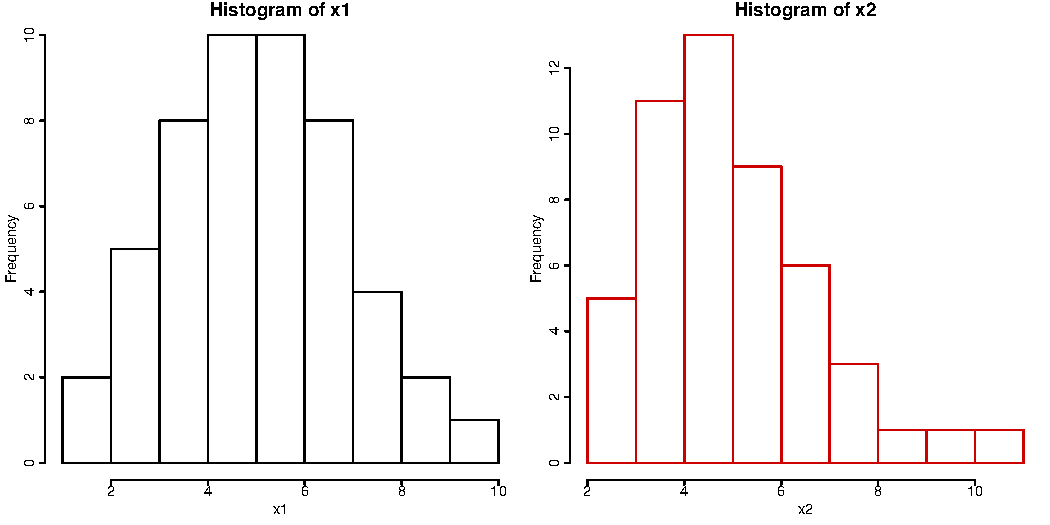
\includegraphics[width=4.5in]{hist1.pdf} %%-Figure (pdf file)
   \vspace{-3ex}
\end{figure}
\end{frame}
%% %%--------------------------------
% \begin{frame}   %%[allowframebreaks]
% \begin{figure}[h]
% %%  %% \centering\includegraphics{BPweibullplot.ps} %%-Figure (ps file)
%    \includegraphics[height=4.5in,angle=90]{CDF1a.pdf} %%-Figure (pdf file)
%    \vspace{-3ex}
% \end{figure}
% \end{frame}
% %% %%--------------------------------
% \begin{frame}   %%[allowframebreaks]
% \begin{figure}[h]
% %%  %% \centering\includegraphics{BPweibullplot.ps} %%-Figure (ps file)
%    \includegraphics[height=3.0in,angle=90]{CDF1b.pdf} %%-Figure (pdf file)
%    \vspace{-3ex}
% \end{figure}
% \end{frame}
%% %%---------------------------------------------------
\begin{frame}   %%[allowframebreaks]
\begin{figure}[h]
%%  %% \centering\includegraphics{BPweibullplot.ps} %%-Figure (ps file)
   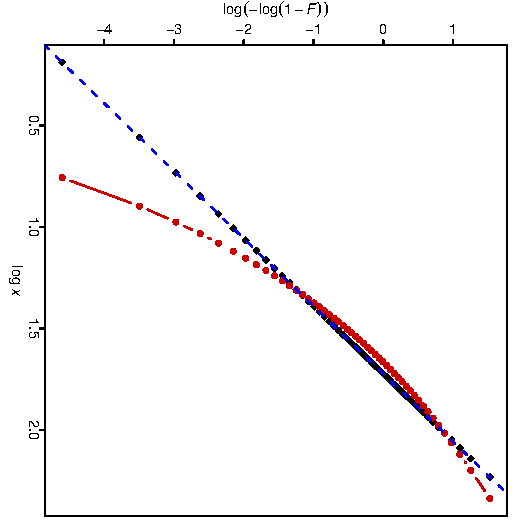
\includegraphics[width=3.0in,angle=90]{Weibull1.pdf} %%-Figure (pdf file)
   \vspace{-3ex}
\end{figure}
\end{frame}
%% %%---------------------------------------------------

